\chapter{Configuring Hbase in Standalone \& Pseudo-distributed mode}
%Intro\footnotemark\\
\par In this Project, we will focus on the use of Hbase with the HDFS file system of
the hadoop ecosystem and with the Spark processing software. So we will use a VM with
Apache Hadoop and Apache Spark installed and configured in local mode.
\begin{spacing}{1.2}
%note en bas de page
\section{Preparating environment }
\par We must first create a VM that is configured with Hadoop2.7.4 (hadoop version compatible with hbase-1.4.7) and with spark-2.4.3 in local mode. Installation and configuration of hadoop and spark on a single node is already from the previous project: INTRODUCTION TO BIG DATA”.\\
We verify that the Hadoop cluster is working fine running the hdfs report command.
\\
\begin{figure}[!htb] 
\begin{center} 
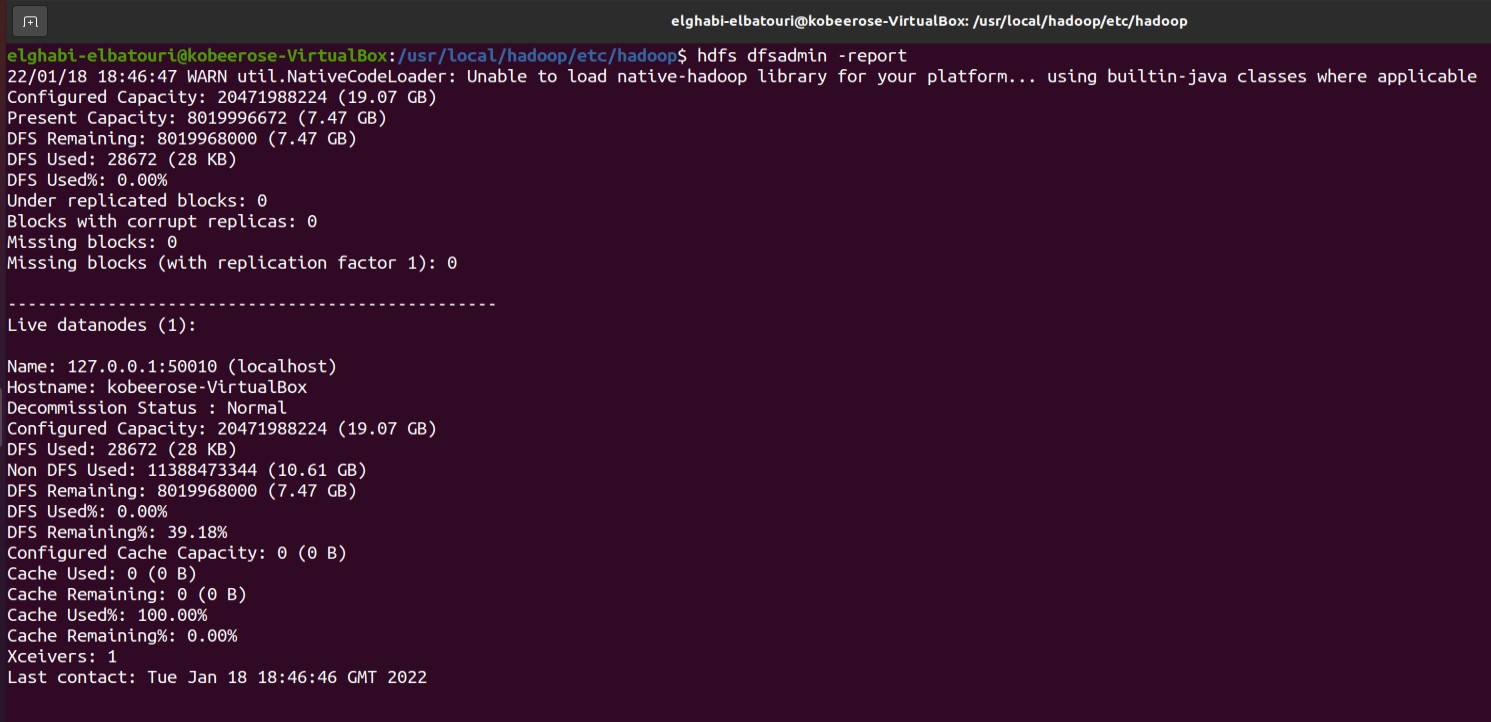
\includegraphics[width=1\linewidth]{Pictures/HBase/Configuring Hbase in Standalone & Pseudo-distributed mode/Preparating environment/hdfs report} 
\end{center} 
\caption{hdfs report} 
\end{figure}  \FloatBarrier
\\
\section{Installing and Configuring Apache Hbase }
\par First Install and configure Hadoop-2.7.4 in single node. We start by downloading HBase.
\\
\begin{figure}[!htb] 
\begin{center} 
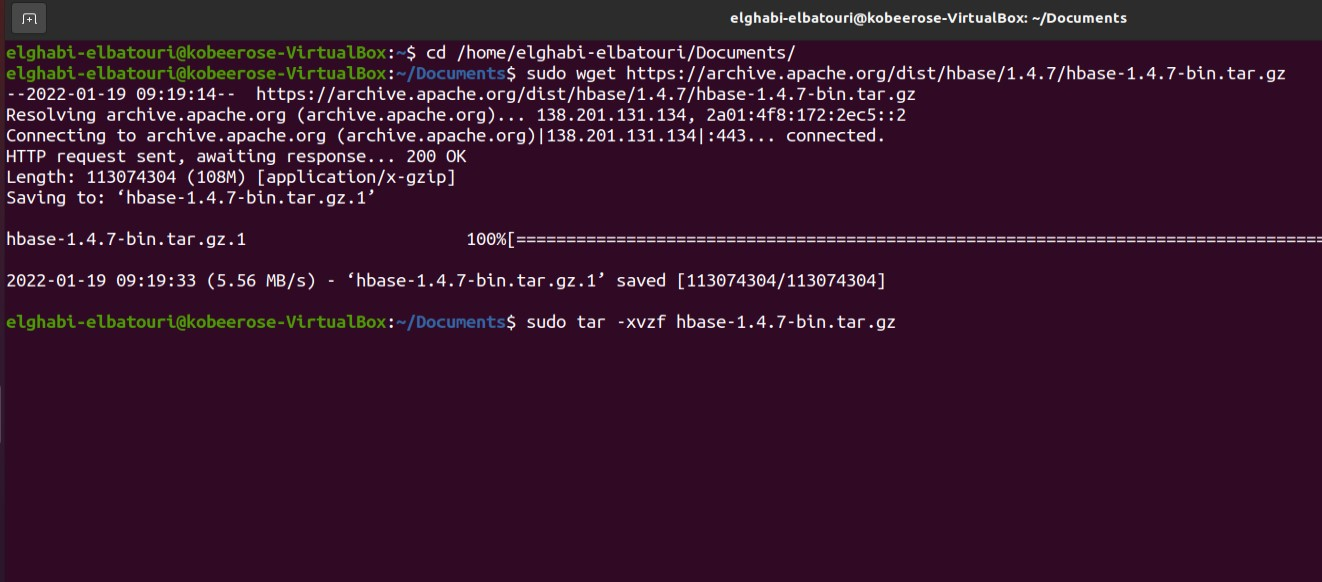
\includegraphics[width=1\linewidth]{Pictures/HBase/Configuring Hbase in Standalone & Pseudo-distributed mode/Installing and Configuring Apache Hbase/Download Hbase} 
\end{center} 
\caption{Download Hbase} 
\end{figure}  \FloatBarrier
\\

\par We rename the created hbase-1.4.7 directory and place it in /usr/local dir.
\\
\begin{figure}[!htb] 
\begin{center} 
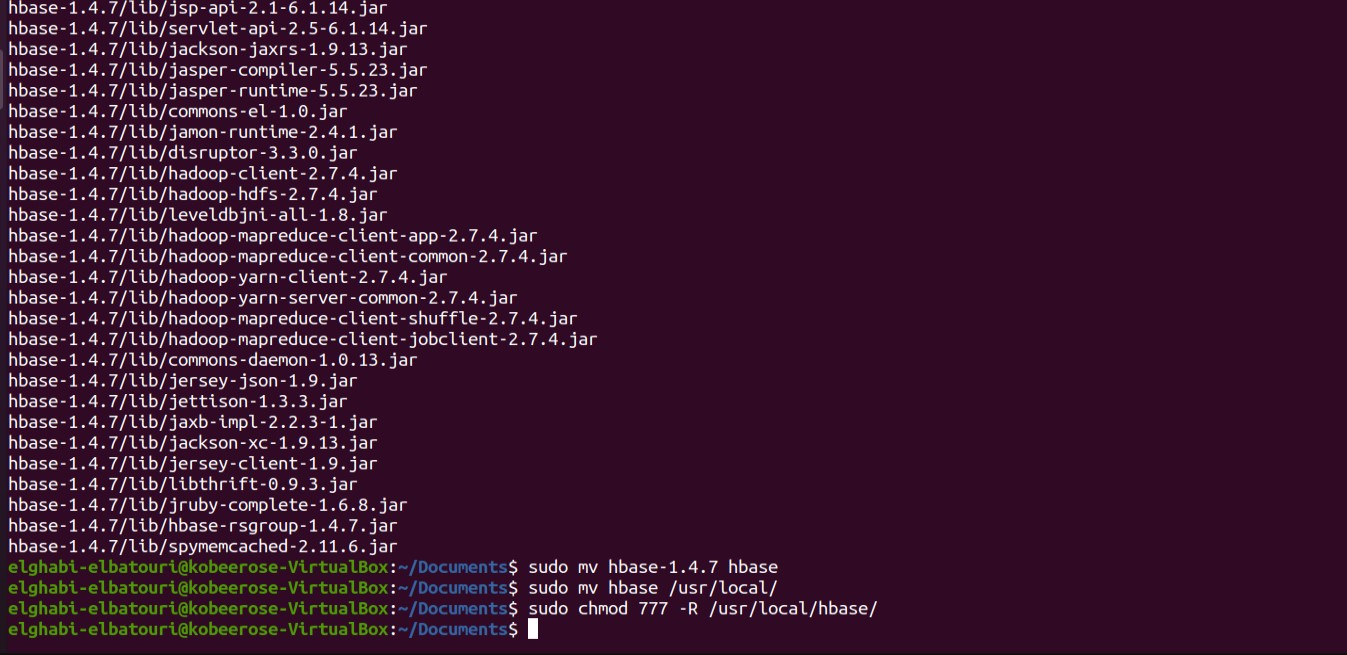
\includegraphics[width=1\linewidth]{Pictures/HBase/Configuring Hbase in Standalone & Pseudo-distributed mode/Installing and Configuring Apache Hbase/Extracting and moving Hbase folder} 
\end{center} 
\caption{Extracting and moving Hbase folder} 
\end{figure}  \FloatBarrier
\\

\par Modifying the PATH by adding the following paths in the .bashrc:
\\
\begin{figure}[!htb] 
\begin{center} 
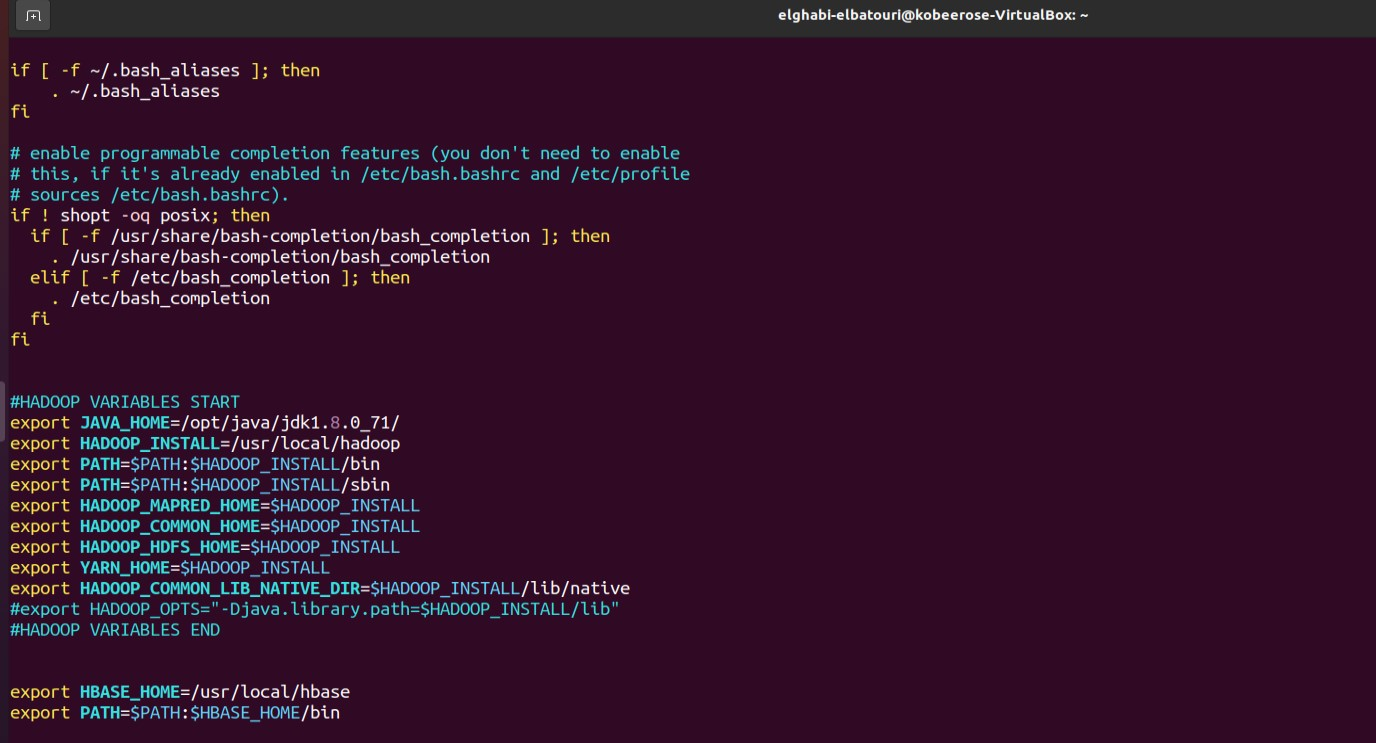
\includegraphics[width=1\linewidth]{Pictures/HBase/Configuring Hbase in Standalone & Pseudo-distributed mode/Installing and Configuring Apache Hbase/Adding Hbase path to .bashrc} 
\end{center} 
\caption{Adding Hbase path to .bashrc} 
\end{figure}  \FloatBarrier
\\

\par Updating the current shell environment source .bashrc commend to apply the changes.
\\
\begin{figure}[!htb] 
\begin{center} 
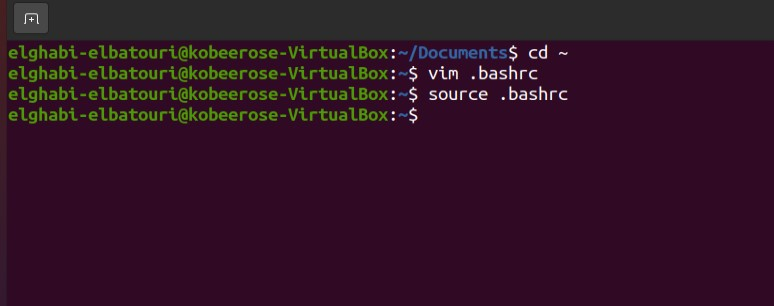
\includegraphics[width=1\linewidth]{Pictures/HBase/Configuring Hbase in Standalone & Pseudo-distributed mode/Installing and Configuring Apache Hbase/Update current shell environment} 
\end{center} 
\caption{Update current shell environment} 
\end{figure}  \FloatBarrier
\\

\par Hbase requires the installation of Java 8. We must install JAVA 8 and after check its installation by typing: java -version.
\\
\begin{figure}[!htb] 
\begin{center} 
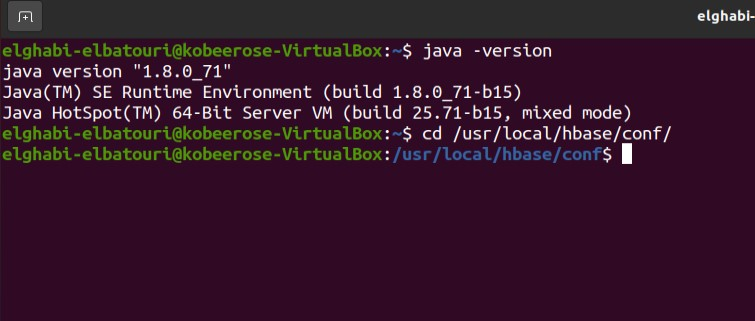
\includegraphics[width=1\linewidth]{Pictures/HBase/Configuring Hbase in Standalone & Pseudo-distributed mode/Installing and Configuring Apache Hbase/Checking Java version} 
\end{center} 
\caption{Checking Java version} 
\end{figure}  \FloatBarrier
\\

\par You must now configure the JAVA\_HOME in the "hbase-env.sh" file.
\\
\begin{figure}[!htb] 
\begin{center} 
\includegraphics[width=1\linewidth]{Pictures/HBase/Configuring Hbase in Standalone & Pseudo-distributed mode/Installing and Configuring Apache Hbase/Adding JAVA\_HOME to hbase-env.sh file} 
\end{center} 
\caption{Adding JAVA\_HOME to hbase-env.sh file} 
\end{figure}  \FloatBarrier
\\

\par Since we will work with a single server, we must modify the /etc/hosts file to change the server address from 127.0.1.1 to 127.0.0.1 as follows:
\\
\begin{figure}[!htb] 
\begin{center} 
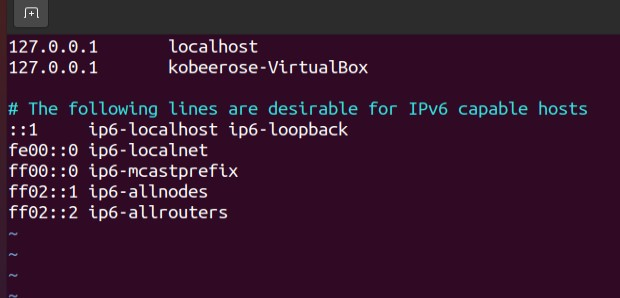
\includegraphics[width=1\linewidth]{Pictures/HBase/Configuring Hbase in Standalone & Pseudo-distributed mode/Installing and Configuring Apache Hbase/Changing IP adresse of host} 
\end{center} 
\caption{Changing IP adresse of host} 
\end{figure}  \FloatBarrier
\\

\par To apply the changes we should restart our machine.
\\
\begin{figure}[!htb] 
\begin{center} 
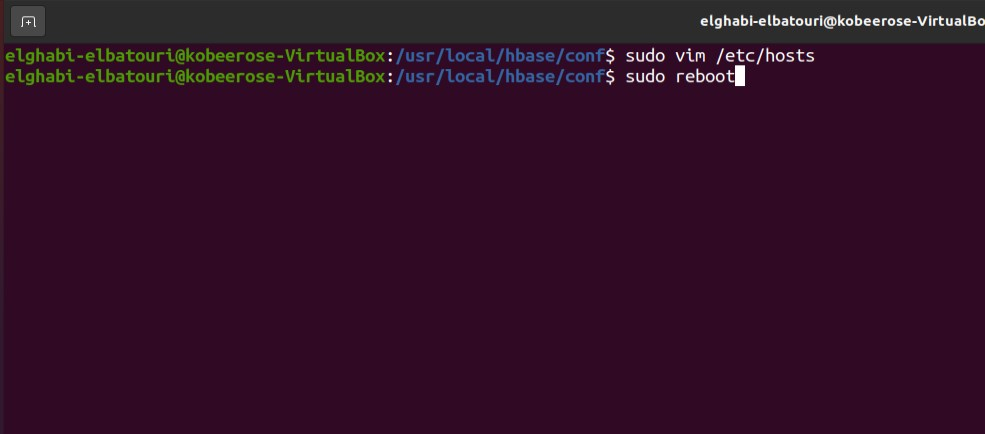
\includegraphics[width=1\linewidth]{Pictures/HBase/Configuring Hbase in Standalone & Pseudo-distributed mode/Installing and Configuring Apache Hbase/rebooting the machine} 
\end{center} 
\caption{Rebooting the machine} 
\end{figure}  \FloatBarrier
\\

\par Let's run the following commands to clean the hadoop\_store in our VM.
\\
\begin{figure}[!htb] 
\begin{center} 
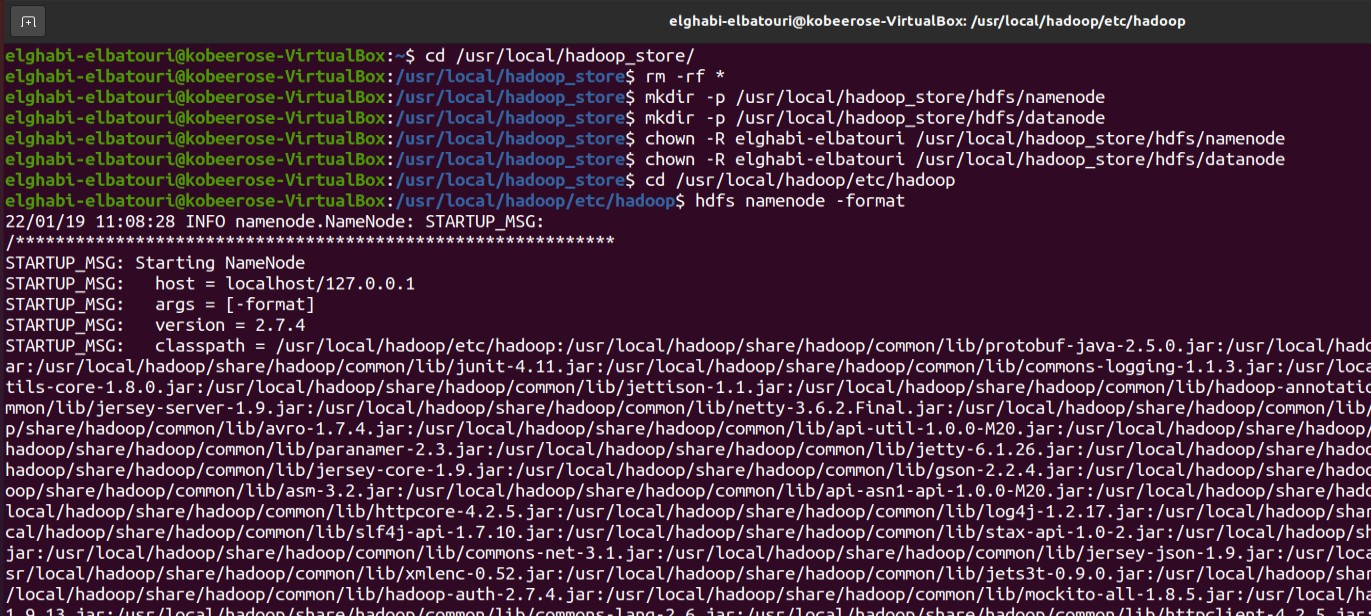
\includegraphics[width=1\linewidth]{Pictures/HBase/Configuring Hbase in Standalone & Pseudo-distributed mode/Installing and Configuring Apache Hbase/Cleaning the hadoop_store} 
\end{center} 
\caption{Cleaning the hadoop\_store} 
\end{figure}  \FloatBarrier
\\

\par Running namenode formatting, starting Hadoop daemons and Verifying that the Hadoop cluster is working.
\\
\begin{figure}[!htb] 
\begin{center} 
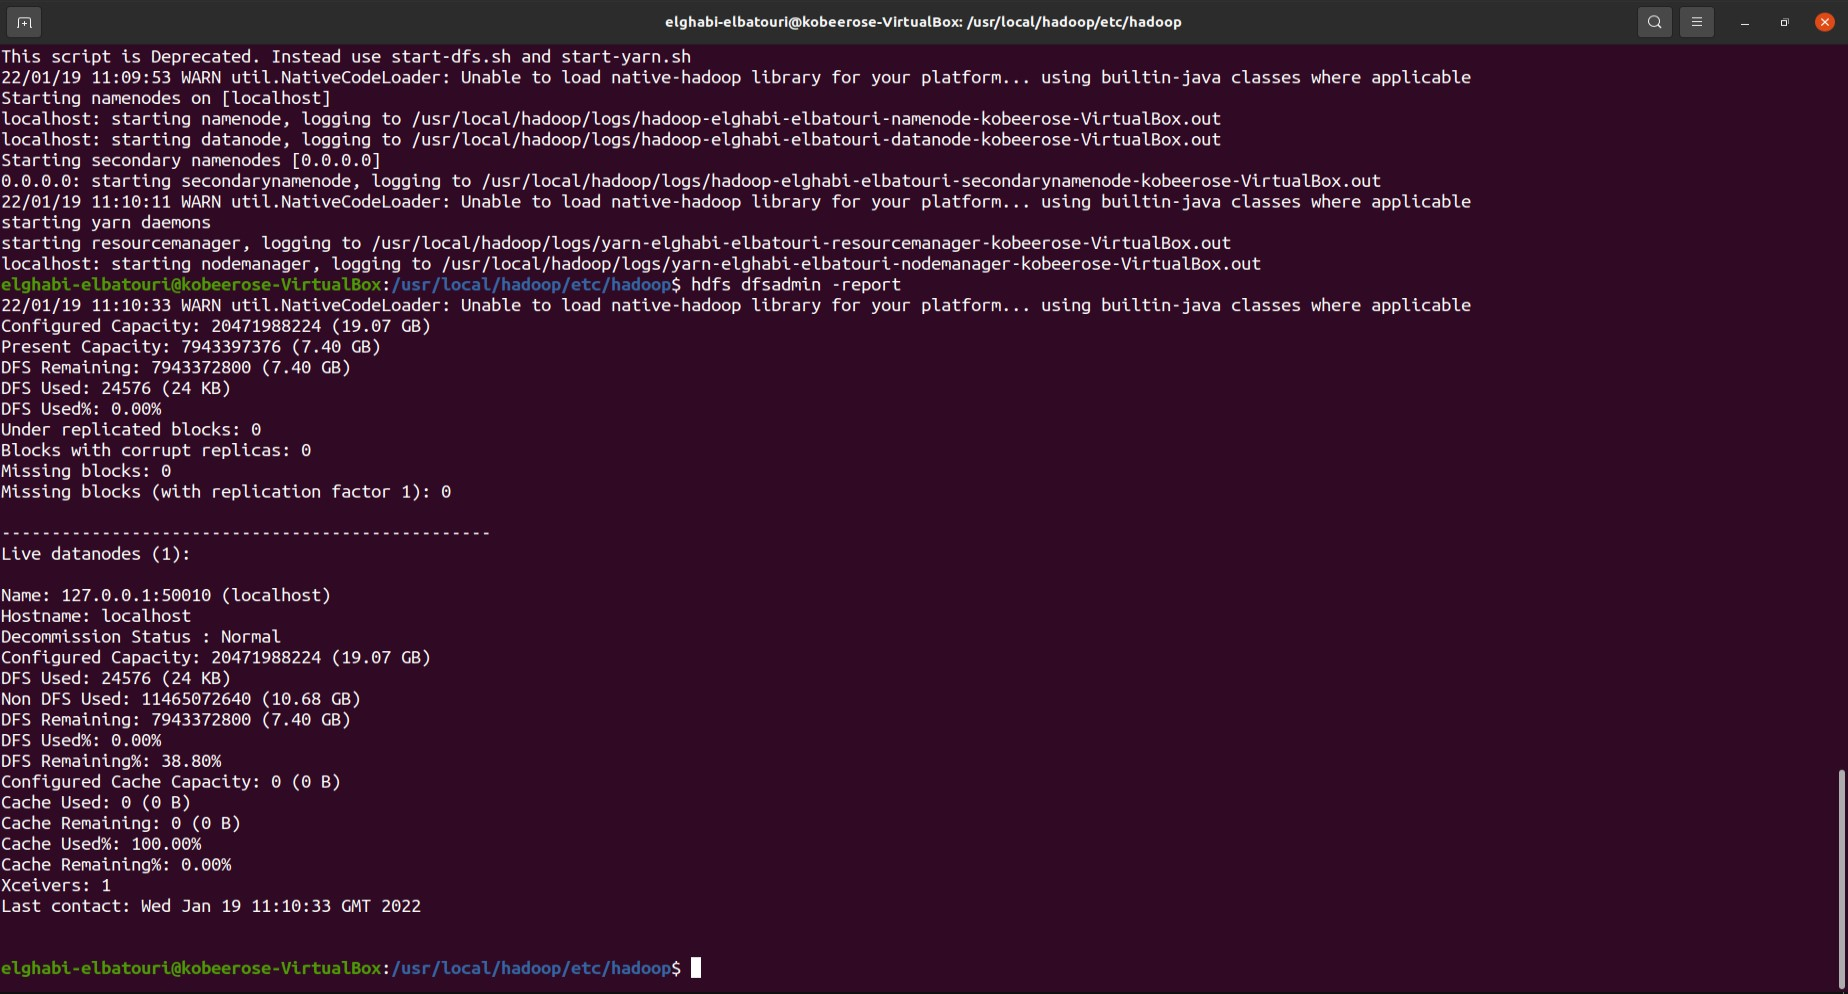
\includegraphics[width=1\linewidth]{Pictures/HBase/Configuring Hbase in Standalone & Pseudo-distributed mode/Installing and Configuring Apache Hbase/Starting hadoop daemons} 
\end{center} 
\caption{Starting hadoop daemons} 
\end{figure}  \FloatBarrier
\\

\section{Configuring Hbase in Standalone mode }

\par In This section will go over the the configuration of a Standalone mode of HBase on a single node. An instance standalone contains all HBase daemons (HMaster and ZooKeeper) running in a single JVM persistent on the local filesystem ( This is the most basic deployment mode ).
\\

\par First, you have to start the Hadoop daemons and make sure they are working.
\\
\begin{figure}[!htb] 
\begin{center} 
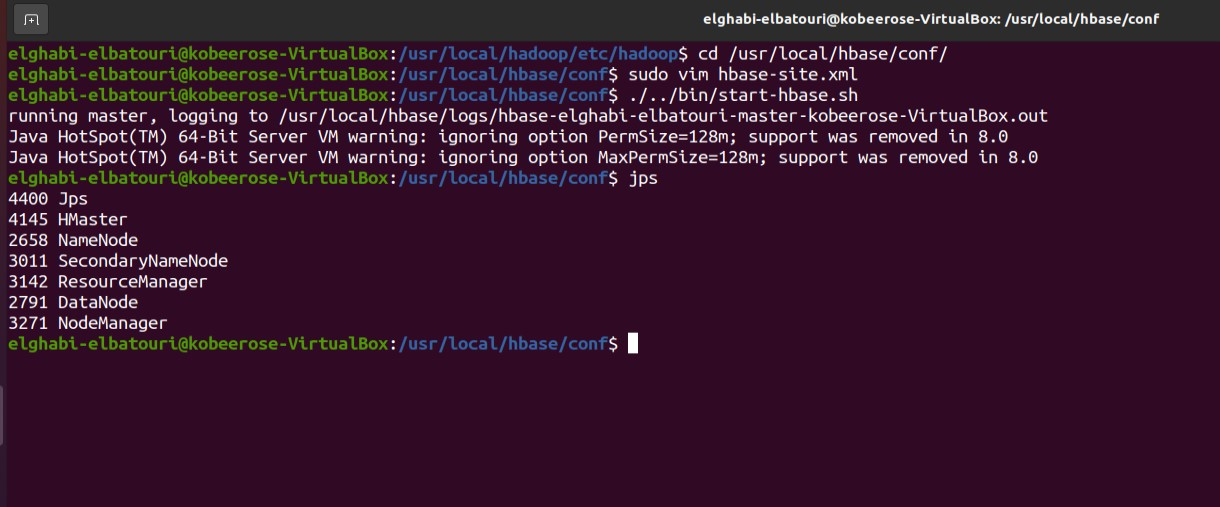
\includegraphics[width=1\linewidth]{Pictures/HBase/Configuring Hbase in Standalone & Pseudo-distributed mode/Configuring Hbase in Standalone mode/HMaster in jps} 
\end{center} 
\caption{HMaster in jps} 
\end{figure}  \FloatBarrier
\\

\par Configuring “hbase-site.xml” for “Standalone” mode.
\\
\begin{figure}[!htb] 
\begin{center} 
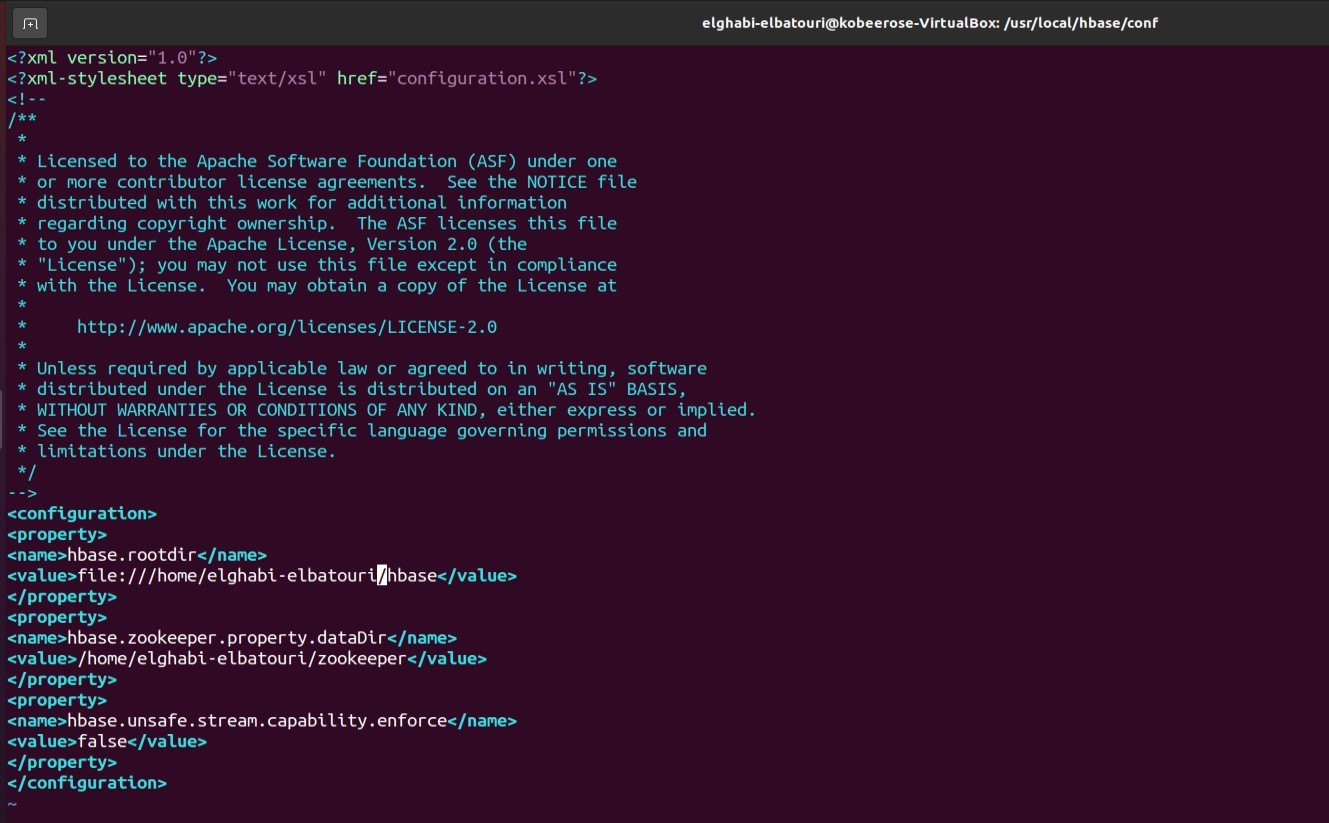
\includegraphics[width=1\linewidth]{Pictures/HBase/Configuring Hbase in Standalone & Pseudo-distributed mode/Configuring Hbase in Standalone mode/Configuration of hbase-site.xml file .jpg} 
\end{center} 
\caption{Configuration of hbase-site.xml file} 
\end{figure}  \FloatBarrier
\\

\par Launching of Hbase in a “Standalone” mode.
\\
\begin{figure}[!htb] 
\begin{center} 
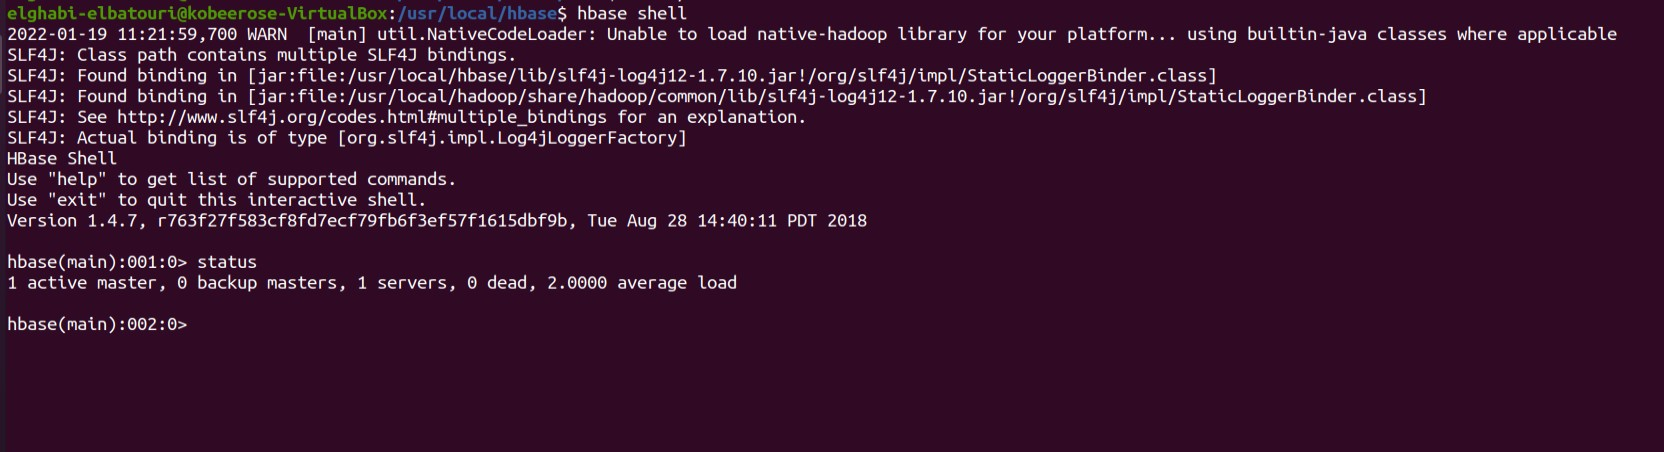
\includegraphics[width=1\linewidth]{Pictures/HBase/Configuring Hbase in Standalone & Pseudo-distributed mode/Configuring Hbase in Standalone mode/Hbase shell} 
\end{center} 
\caption{Hbase shell} 
\end{figure}  \FloatBarrier
\\

\par Stopping all Hbase daemons bt typing stop-hbase.sh
\\
\begin{figure}[!htb] 
\begin{center} 
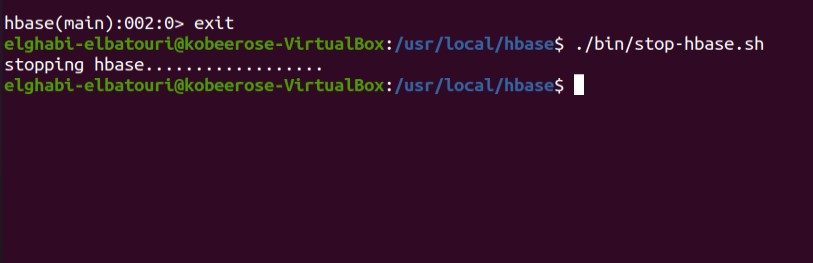
\includegraphics[width=1\linewidth]{Pictures/HBase/Configuring Hbase in Standalone & Pseudo-distributed mode/Configuring Hbase in Standalone mode/Stopping Hbase daemons} 
\end{center} 
\caption{Stopping Hbase daemons} 
\end{figure}  \FloatBarrier
\\


\section{Configuring Hbase in Pseudo-distributed mode }
\par This section describes the configuration of a "pseudo-distributed" mode. Since we are using a single node (a single VM), hbase then runs on a single node, which means that each HBase daemon (HMaster,HRegionServer and ZooKeeper) will run as a separate process in the node (using multi threading).
\\

\par Creation of the necessary files for Hbase in the HDFS starting by Hbase's repositories in Hadoop.
\\
\begin{figure}[!htb] 
\begin{center} 
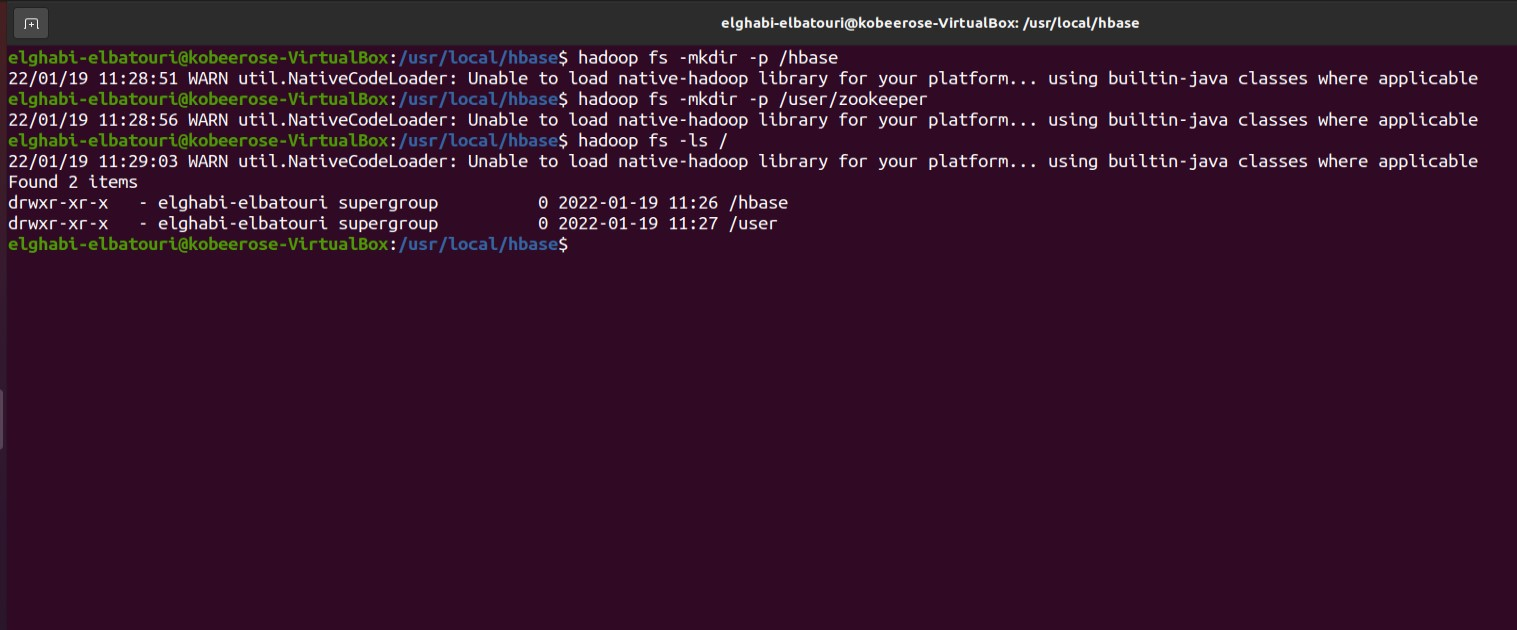
\includegraphics[width=1\linewidth]{Pictures/HBase/Configuring Hbase in Standalone & Pseudo-distributed mode/Configuring Hbase in Standalone mode/Creating Hbase repositories in Hadoop} 
\end{center} 
\caption{Creating Hbase repositories in Hadoop} 
\end{figure}  \FloatBarrier
\\

\par we should also confugure HBase in pseudo-distributed mode by adding the following lines in the “hbase-site.xml”
\\
\begin{figure}[!htb] 
\begin{center} 
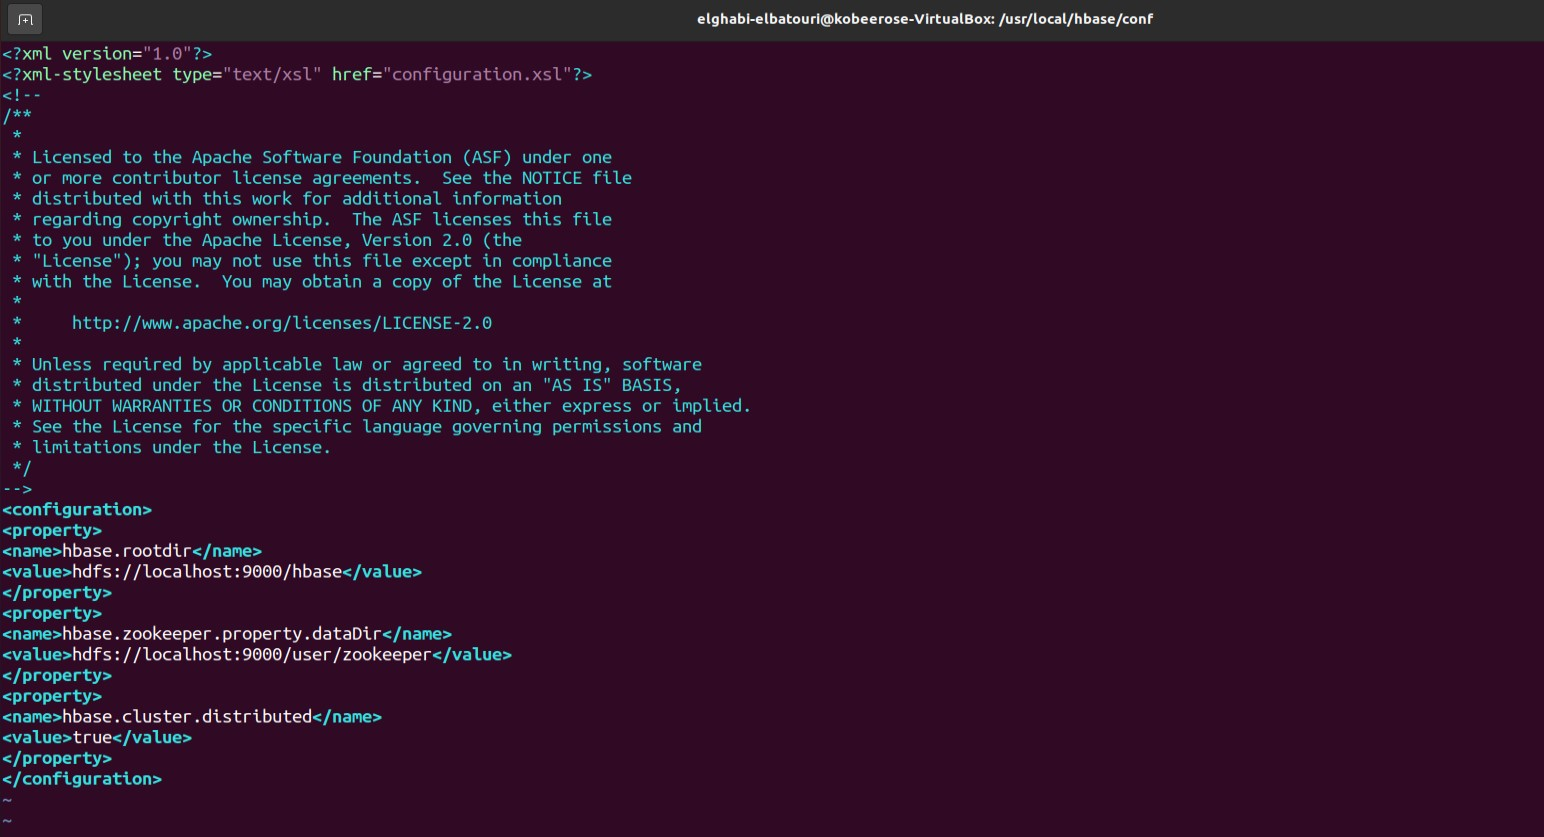
\includegraphics[width=1\linewidth]{Pictures/HBase/Configuring Hbase in Standalone & Pseudo-distributed mode/Configuring Hbase in Pseudo-distributed mode/Configuring hbase-site.xml for Distributed mode} 
\end{center} 
\caption{Configuring hbase-site.xml for Distributed mode} 
\end{figure}  \FloatBarrier
\\

\par Now let's launch Hbase and verify that all services are working with the jps command.
\\
\begin{figure}[!htb] 
\begin{center} 
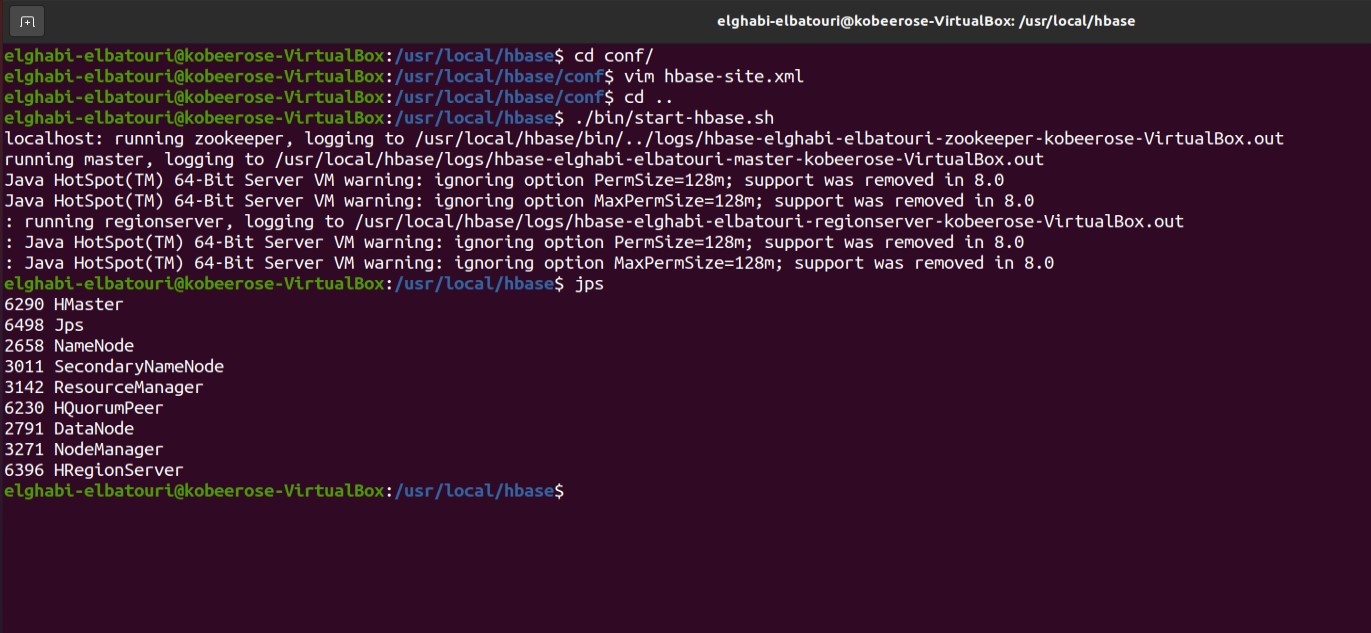
\includegraphics[width=1\linewidth]{Pictures/HBase/Configuring Hbase in Standalone & Pseudo-distributed mode/Configuring Hbase in Pseudo-distributed mode/Launching Hbase} 
\end{center} 
\caption{Launching Hbase} 
\end{figure}  \FloatBarrier
\\

\par We can check Hbase status in our browser by going the to localhost:16010/master-status
 url.
\\
\begin{figure}[!htb] 
\begin{center} 
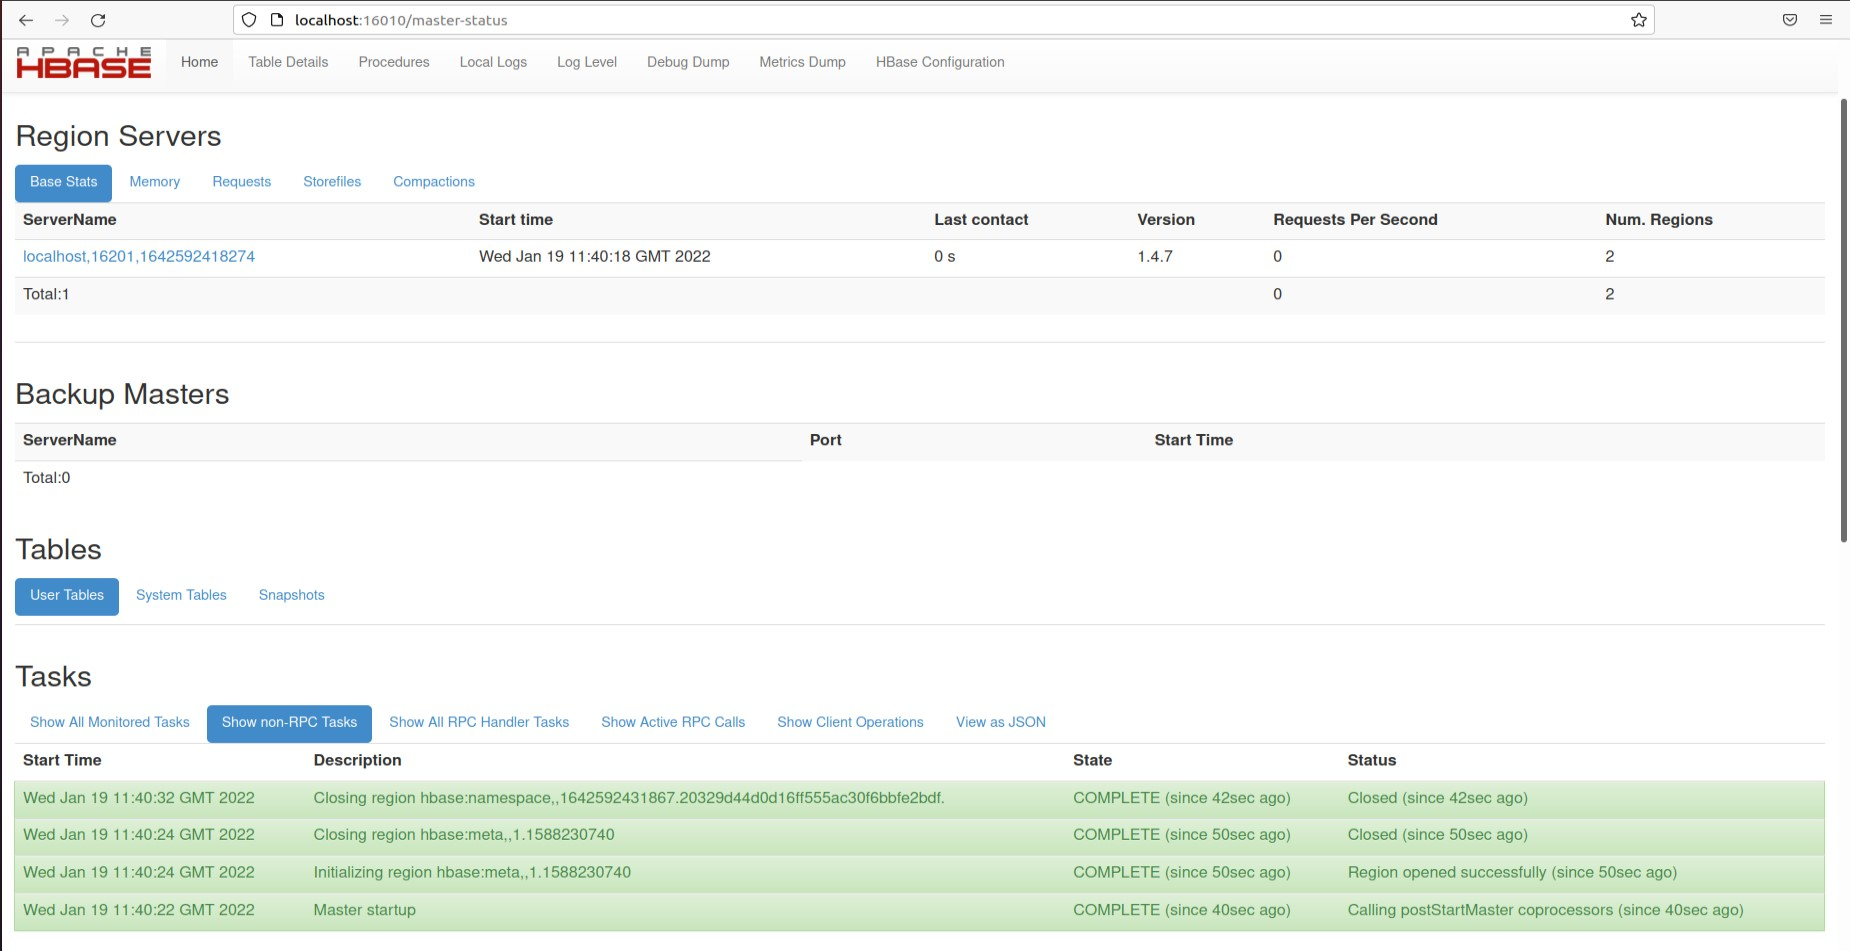
\includegraphics[width=1\linewidth]{Pictures/HBase/Configuring Hbase in Standalone & Pseudo-distributed mode/Configuring Hbase in Pseudo-distributed mode/Testing in browser} 
\end{center} 
\caption{Testing in browser} 
\end{figure}  \FloatBarrier
\\

\par We can Also test Hbase terminal.
\\
\begin{figure}[!htb] 
\begin{center} 
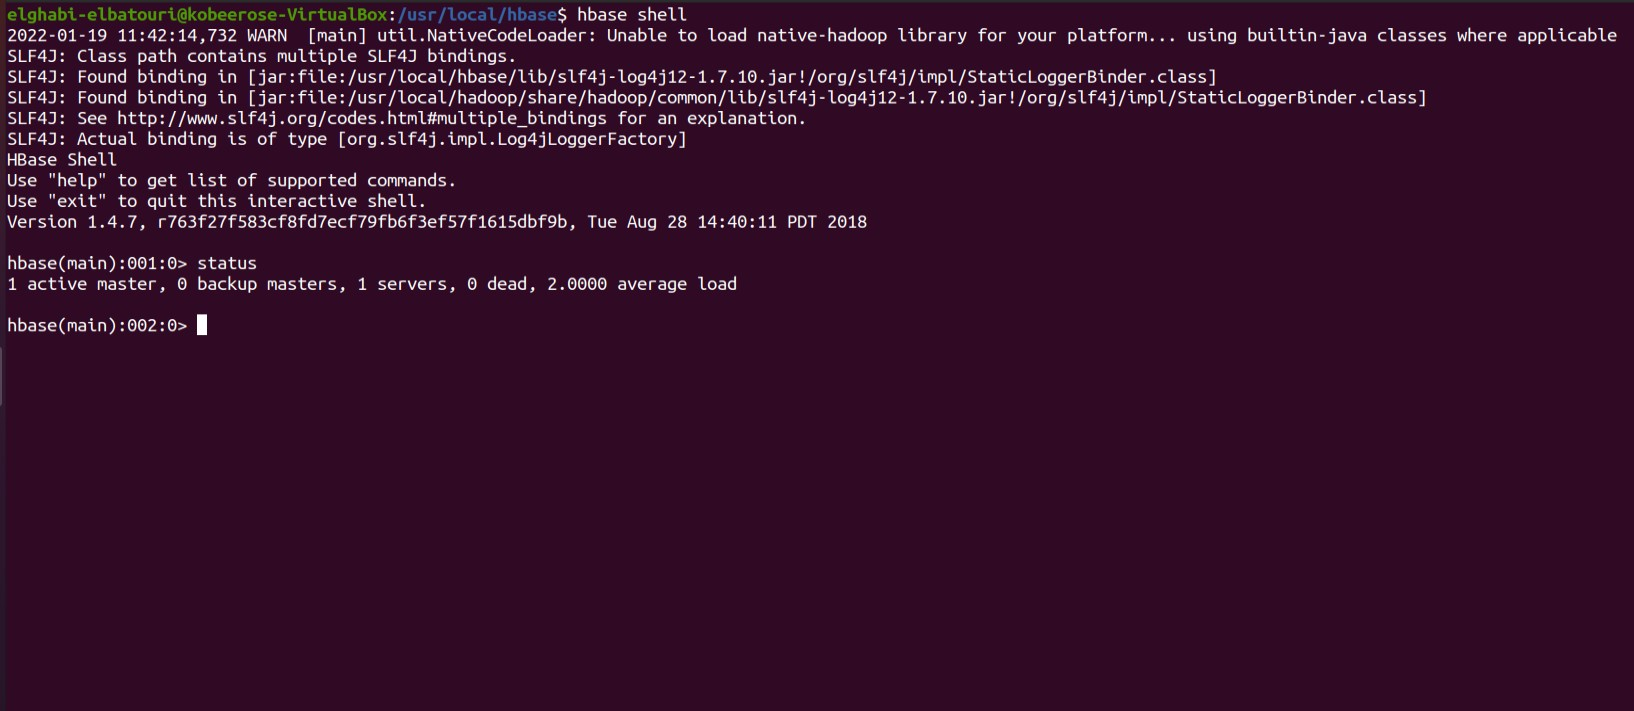
\includegraphics[width=1\linewidth]{Pictures/HBase/Configuring Hbase in Standalone & Pseudo-distributed mode/Configuring Hbase in Pseudo-distributed mode/Testing in Terminal} 
\end{center} 
\caption{Testing in Terminal} 
\end{figure}  \FloatBarrier
\\

\end{spacing}